% Pollis drill-down: the data packages PollisDatasets.jl, PollisJournals.jl, PollisReferences.jl and PollisRSS.jl,
% and how the user's own data lives beside them (25 October 2026).
% For users who want the detail, and for whoever maintains Pollis.
% Compile with: latexmk -pdf workflow_data_packages.tex
% Shared look for the one-page Pollis workflow handouts (same fonts and colours as the brochure).
\documentclass[10pt,a4paper]{article}

\usepackage[a4paper,left=17mm,right=17mm,top=14mm,bottom=16mm,footskip=8mm]{geometry}
\usepackage[T1]{fontenc}
\usepackage[default,semibold]{sourcesanspro}
\usepackage{microtype}
\usepackage{graphicx}
\usepackage[table]{xcolor}
\usepackage{tikz}
\usepackage[most]{tcolorbox}
\usepackage{fontawesome5}
\usepackage{enumitem}
\usepackage{fancyhdr}
\usepackage[hidelinks]{hyperref}

\graphicspath{{images/}}

% ---------------------------------------------------------------- colours (as in the brochure)
\definecolor{navy}{HTML}{1C3A5E}
\definecolor{pblue}{HTML}{3B78B5}
\definecolor{amber}{HTML}{F2B33D}
\definecolor{deepamber}{HTML}{D9902A}
\definecolor{pale}{HTML}{EEF3F9}
\definecolor{ink}{HTML}{2A2F36}
\definecolor{logonavy}{HTML}{173D63}
\definecolor{logodark}{HTML}{C98A1E}
\definecolor{logoamber}{HTML}{F2B446}
\definecolor{logocream}{HTML}{FEEFD2}
\definecolor{soft}{HTML}{5E6773}
\color{ink}

\setlength{\parindent}{0pt}
\setlength{\parskip}{3pt}
\setlist{nosep,leftmargin=*,itemsep=2pt}

\pagestyle{fancy}
\fancyhf{}
\renewcommand{\headrulewidth}{0pt}
\fancyfoot[L]{\footnotesize\color{soft}\textbf{Pollis}\enspace Bright Insights through Statistical Learning, Simulation and Optimisation}
\fancyfoot[R]{\footnotesize\color{soft}github.com/saragga/pollis/releases/latest}

% The Pollis logo, redrawn so it prints sharply at any size
\newcommand{\pollislogo}[1]{%
  \begin{tikzpicture}[x=#1/512,y=-#1/512,baseline=(current bounding box.center)]
    \fill[logonavy] (0,0) rectangle (512,512);
    \fill[logodark] (36,422) -- (104,256) -- (172,422) -- cycle;
    \fill[logoamber] (104,422) -- (203,180) -- (302,422) -- cycle;
    \fill[logocream] (203,422) -- (339,89) -- (476,422) -- cycle;
  \end{tikzpicture}}

% Top of the page: logo, name, kind of document (Workflow unless given, e.g. [Drill-Down]) and its subject;
% then the question and a one-line promise
\newcommand{\workflowhead}[4][Workflow]{%
  \thispagestyle{fancy}%
  \begin{minipage}[c]{13mm}\pollislogo{11mm}\end{minipage}%
  \begin{minipage}[c]{\dimexpr\linewidth-13mm\relax}
    {\color{navy}\Large\bfseries Pollis}\enspace{\color{soft}#1}\hfill
    {\color{deepamber}\small\bfseries\MakeUppercase{#2}}
  \end{minipage}\par\vspace{7mm}
  {\color{navy}\fontsize{22}{26}\selectfont\bfseries #3}\par\vspace{4pt}
  {\color{soft}\large #4}\par\vspace{5mm}}

% A menu path: \menu{Explore}{Access Data Libraries}... is written as \path{Explore \gt Access Data Libraries}
\newcommand{\gt}{\,{\color{deepamber}\bfseries ›}\,}
\newcommand{\menupath}[1]{{\footnotesize\bfseries\color{navy}#1}}

% A screenshot if images/<file> exists, otherwise an orange placeholder that says what to capture
\newlength{\shotheight}\setlength{\shotheight}{43mm}
\newcommand{\stepshot}[2]{%
  \IfFileExists{images/#1}{%
    \tcbox[enhanced, colback=black, colframe=black!70, boxrule=0.4pt, arc=2pt,
      left=0pt,right=0pt,top=0pt,bottom=0pt, boxsep=0pt, halign=center]{%
      \includegraphics[width=\dimexpr\linewidth-1pt\relax,height=\shotheight,keepaspectratio]{#1}}}{%
    \begin{tcolorbox}[enhanced, colback=white, colframe=orange!80, boxrule=0.6pt, arc=2pt,
      height=\shotheight, valign=center, halign=center, left=6pt, right=6pt]
      {\color{orange}\Large\faCamera}\par\smallskip
      {\color{orange}\footnotesize\bfseries Screenshot: #2}\par\smallskip
      {\color{orange!80!black}\scriptsize images/#1}
    \end{tcolorbox}}}

% One step: number, title, menu path, image file, what to capture, what it means
\newcommand{\step}[6]{%
  \begin{tcolorbox}
    {\color{deepamber}\Large\bfseries #1}\enspace{\color{navy}\large\bfseries #2}\par\vspace{1pt}
    \menupath{#3}\par\vspace{4pt}
    \stepshot{#4}{#5}\par\vspace{3pt}
    {\small #6}
  \end{tcolorbox}}

\newenvironment{steps}{%
  \begin{tcbraster}[raster columns=2, raster equal height=rows, raster column skip=4mm,
    raster row skip=4mm, enhanced, colback=pale, colframe=pale, boxrule=0pt, sharp corners,
    left=6pt,right=6pt,top=6pt,bottom=6pt, fontupper=\raggedright]}{\end{tcbraster}}

% Boxes for the bottom of the page
\newtcolorbox{pbox}[2][]{enhanced, colback=pale, colframe=amber, boxrule=0pt,
  leftrule=3pt, sharp corners, left=7pt, right=7pt, top=6pt, bottom=6pt,
  fontupper=\small\raggedright, before upper={{\color{navy}\normalsize\bfseries #2}\par\smallskip}, #1}
\newtcolorbox{nbox}[1][]{enhanced, colback=navy, colframe=navy, boxrule=0pt,
  sharp corners, left=8pt, right=8pt, top=6pt, bottom=6pt, coltext=white,
  fontupper=\small\raggedright, #1}

% A Next Steps item inside the bottom boxes
\newcommand{\nsitem}[2]{\item[\color{deepamber}\faChevronRight] \textbf{#1}: #2}


\usepackage{titlesec}
\usepackage{tabularx}
\usepackage{booktabs}
\usepackage{listings}
\usetikzlibrary{positioning,arrows.meta,fit}

\fancyhf{}
\fancyfoot[L]{\footnotesize\color{soft}\textbf{Pollis}\enspace Drill-down: data packages}
\fancyfoot[R]{\footnotesize\color{soft}\thepage}

\titleformat{\section}{\color{navy}\large\bfseries}{\color{deepamber}\thesection}{0.6em}{}
\titleformat{\subsection}{\color{navy}\normalsize\bfseries}{\color{deepamber}\thesubsection}{0.5em}{}
\titlespacing*{\section}{0pt}{12pt}{4pt}
\titlespacing*{\subsection}{0pt}{8pt}{2pt}
\setlength{\parskip}{4pt}

\lstset{basicstyle=\ttfamily\footnotesize, columns=fullflexible, keepspaces=true, breaklines=true,
  backgroundcolor=\color{pale}, frame=leftline, rulecolor=\color{amber}, framerule=2pt, xleftmargin=6pt,
  framexleftmargin=6pt, aboveskip=4pt, belowskip=4pt, upquote=true, tabsize=2}

\usepackage{xurl}
\newcommand{\file}[1]{{\small\nolinkurl{#1}}}
\newcolumntype{L}{>{\raggedright\arraybackslash}X}

\begin{document}

\workflowhead[Drill-Down]{Data Packages}
  {The data of Pollis, and yours beside it}
  {PollisDatasets.jl, PollisJournals.jl, PollisReferences.jl and PollisRSS.jl: what each holds, how it reaches your
   computer and becomes a database, how it is updated without a new Pollis, and how the data you add lives beside it
   without ever being touched.}

\begin{nbox}
{\color{amber}\bfseries Drill-down.}\enspace
A look under the surface of what the Guide describes in \emph{Data and Databases} and \emph{Built-in Databases}. It is
for anyone who wants to know where their data is and why it is safe, and for whoever maintains Pollis
(\S\ref{sec:procedures} is for them). It describes the state of 25 October 2026.
\end{nbox}

\tableofcontents

\section{The data layer in one table}

Pollis is a program; the data it comes with is not part of it. Four Julia packages on GitHub hold that data, each
changing on its own timetable, so a new dataset, a new month of journals, a corrected DOI or a new feed reaches you
without a new Pollis.

\begin{center}\small
\renewcommand{\arraystretch}{1.25}
\begin{tabularx}{\linewidth}{@{}p{0.15\linewidth}LLLL@{}}
\toprule
& \textbf{PollisDatasets.jl} & \textbf{PollisJournals.jl} & \textbf{PollisReferences.jl} & \textbf{PollisRSS.jl}\\
\midrule
Holds & 65 real datasets and 2 simulated, each with its source, licence and columns & 251,461 journals, conferences and series; the Norwegian register & 650 works Pollis cites, 797 dated citation counts & 519 feeds under 35 topics\\
Form & CSV files and \file{datasets.toml} & Parquet files in a Julia artifact & one JSON file & one JSON file\\
Changes & when a dataset is added & monthly, by a workflow & when a work is corrected or cited & when a feed is added or corrected\\
Database & PollisDatasets & PollisJournals & PollisReferences & PollisRSS\\
In Julia & \file{pollis} & \file{journals} & \file{references} & \file{rss}\\
Reaches Pollis & install road & install road & install and build roads & install and build roads\\
Licence & code MIT; each dataset its own & code MIT; data CC0 and NLOD 2.0 & MIT & MIT\\
\bottomrule
\end{tabularx}
\end{center}

All four live under \file{github.com/Trumpingtons}, all are installed by URL, not from the General registry, and
Pollis follows the latest \emph{commit} of their \file{main}, not version numbers (which are chosen by hand; Pollis
does not use semver).

\section{The principle: Pollis's data is replaceable, yours never}\label{sec:principle}

Three rules, and everything else follows from them.
\begin{enumerate}
  \item \textbf{What a package brings is a copy that an update may replace.} Pollis never asks you to look after it.
  \item \textbf{What you do is written to files of yours that no update writes.} They are JSON Lines, appended to and
    never rewritten: a change is a new line, and for each key \emph{the last line wins}.
  \item \textbf{The five built-in databases are builds over both}, read-only, rebuilt when what they come from
    changes. Deleting one loses nothing: it is made again at the next start of the Julia REPL.
\end{enumerate}

\begin{center}\small
\renewcommand{\arraystretch}{1.25}
\begin{tabularx}{\linewidth}{@{}p{0.45\linewidth}L@{}}
\toprule
\textbf{Pollis's, replaced by updates} & \textbf{Yours, never replaced}\\
\midrule
the installed packages, in \file{~/.pollis/julia/environments/v1.13} & your own databases, wherever you keep them\\
\file{~/.pollis/databases/*.duckdb} and their \file{.stamp} files & \file{~/.pollis/journals/metrics/*.jsonl}, the metrics you imported\\
\file{~/.pollis/databases/PollisDatasets.json} & \file{~/.pollis/journals/articles.jsonl}, articles looked up\\
\file{~/.pollis/journals/scores.csv} & \file{~/.pollis/references/references.jsonl}, \file{counts.jsonl}, \file{versions.jsonl}, \file{panels.jsonl}\\
\file{~/.pollis/references/pollis.json}, \file{package.json} & \file{~/.pollis/rss/feeds.jsonl}, \file{items/*.jsonl}, \file{zotero.jsonl}, \file{episodes.jsonl}\\
\file{~/.pollis/rss/catalogue.json} & the RSS settings: unsubscribed, removed, hidden, welcome page\\
\bottomrule
\end{tabularx}
\end{center}

\section{The whole flow at a glance}

\begin{center}
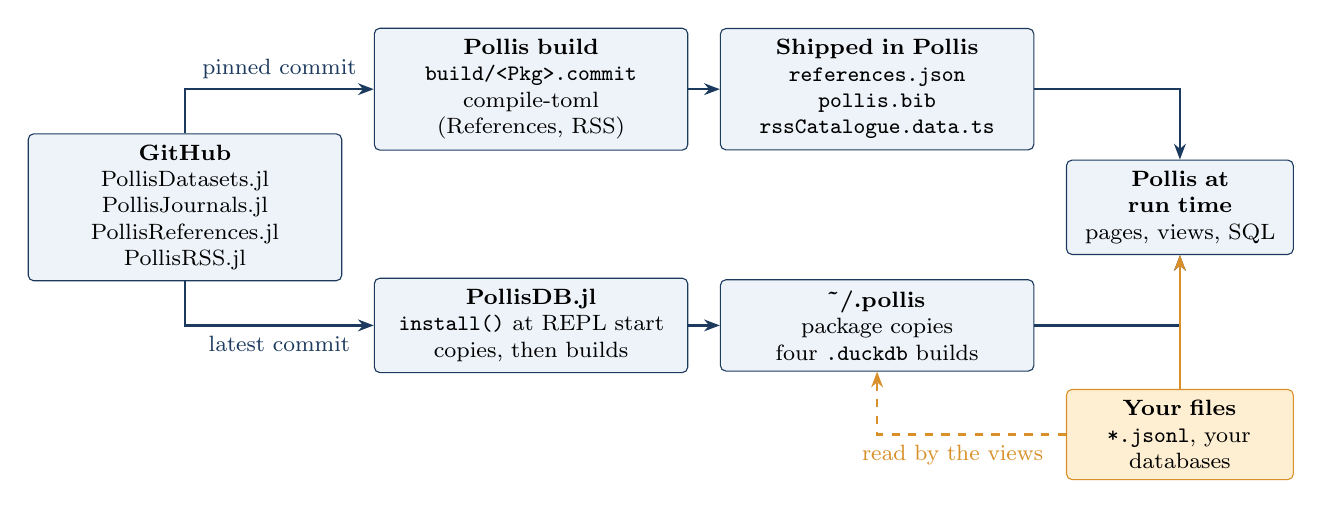
\begin{tikzpicture}[font=\footnotesize, node distance=5mm and 4mm,
  box/.style={draw=navy, fill=pale, rounded corners=2pt, align=center, inner sep=4pt, text width=37mm},
  user/.style={box, draw=deepamber, fill=logocream},
  arr/.style={-{Stealth[length=2mm]}, navy, thick}]
  \node[box] (repo) {\textbf{GitHub}\\PollisDatasets.jl\\PollisJournals.jl\\PollisReferences.jl\\PollisRSS.jl};
  \node[box, right=of repo, yshift=15mm] (pin) {\textbf{Pollis build}\\\texttt{build/<Pkg>.commit}\\compile-toml\\(References, RSS)};
  \node[box, right=of pin] (ship) {\textbf{Shipped in Pollis}\\\texttt{references.json}\\\texttt{pollis.bib}\\\texttt{rssCatalogue.data.ts}};
  \node[box, right=of repo, yshift=-15mm] (install) {\textbf{PollisDB.jl}\\\texttt{install()} at REPL start\\copies, then builds};
  \node[box, right=of install] (copy) {\textbf{\textasciitilde/.pollis}\\package copies\\four \texttt{.duckdb} builds};
  \node[box, right=of ship, yshift=-15mm, text width=26mm] (app) {\textbf{Pollis at run time}\\pages, views, SQL};
  \node[user, below=of app, yshift=-12mm, text width=26mm] (mine) {\textbf{Your files}\\\texttt{*.jsonl}, your databases};
  \draw[arr] (repo) |- node[pos=0.75, above] {pinned commit} (pin);
  \draw[arr] (pin) -- (ship);
  \draw[arr] (repo) |- node[pos=0.75, below] {latest commit} (install);
  \draw[arr] (install) -- (copy);
  \draw[arr] (ship) -| (app);
  \draw[arr] (copy) -| (app);
  \draw[arr, deepamber] (mine) -- (app);
  \draw[arr, deepamber, dashed] (mine.west) -| node[pos=0.3, below] {read by the views} (copy.south);
\end{tikzpicture}
\end{center}

Two roads lead from a package to you. The \emph{install road} takes the newest commit on GitHub through the Julia
REPL, copies what Pollis's pages read, and builds the databases; all four packages take it. The \emph{build road}
takes PollisReferences.jl and PollisRSS.jl at a commit pinned in the Pollis repository and bakes them into every
Pollis, because the References and RSS pages must work in a Pollis without Julia, offline, or on its very first start.
PollisDatasets and PollisJournals need no build road: they are only ever read through Julia and DuckDB. Your files
reach the pages directly, and reach the databases through views that read them whenever they are queried.

\section{\texorpdfstring{PollisDB.jl}{PollisDB.jl}: the Julia side of Pollis}\label{sec:pollisdb}

The four packages are data; what installs them, builds the databases and connects you to them is
\file{PollisDB.jl}. It is not a package: it is a Julia module inside Pollis itself, in its Julia extension
(\file{extensions/language-julia/scripts/terminalserver/PollisDB.jl}), under Pollis's licence, AGPL-3.0. Every time
the Julia REPL starts, Pollis loads it into the REPL as \file{PollisDB}, so it is always there, in any project, without
being added to it. It has four jobs.
\begin{enumerate}
  \item \textbf{Keep the data packages installed and current} (\file{install()}, \file{needs_install()}): it adds
    the four packages, and DuckDB, to an environment of Pollis's own, \file{~/.pollis/julia/environments/v1.13}, and
    updates them when GitHub has newer commits. That environment is on the load path, so \file{using DuckDB} or
    \file{using PollisDatasets} works in any of your projects without touching its \file{Project.toml}.
  \item \textbf{Build the four databases} (\file{build()}, \file{build_journals()}, \file{build_references()},
    \file{build_rss()}), and copy the data files that Pollis's pages read (\file{copy_package_data()}). The fifth,
    PollisDocuments, the passages Ask Pollis searches, is made by the Julia extension's \file{ask_index.jl} once the
    documents are compiled.
  \item \textbf{Connect} (\file{connect()}, \file{sql()}, the \file{sql>} mode): a DuckDB connection with the five
    built-in databases attached read-only, and DuckDB's full-text search extension, fts, loaded.
  \item \textbf{Feed the Databases view} (\file{show()}, \file{register()}): each connection handed to it is
    described, schemas, tables and columns, in a JSON file in \file{~/.pollis/databases/sessions}, which the view
    watches.
\end{enumerate}
Its DuckDB is Pollis's fork of DuckDB.jl, \file{github.com/Trumpingtons/DuckDB.jl}, which brings no engine of its own:
it loads the one Pollis ships, copied to \file{~/.pollis/duckdb} with the fts extension, so every DuckDB in Pollis,
the \file{duckdb>} terminal included, is the same engine.

\section{The four packages}

\subsection{PollisDatasets.jl: the datasets of the examples}
\textbf{What it holds.} 65 small, real datasets and 2 simulated ones, from \file{mtcars} and \file{iris} to \file{mroz} and
\file{challenger}, grouped by domain (Regression, Time Series, \ldots), that the Code Examples of Pollis load. Each is
\file{data/<id>.csv} with an entry in \file{datasets.toml}:
\begin{lstlisting}
[[datasets]]
id = "mtcars"
title = "Motor Trend Cars"
domain = "Regression"
description = "Fuel consumption and ten design and performance variables for 32 cars (1973-74 models)."
rows = 32
source = "Henderson, H. V. and Velleman, P. F. (1981), Building multiple regression models interactively, ..."
url = "R datasets package (mtcars)"
licence = "None stated; R datasets package (GPL-2 | GPL-3)"
status = "redistributed"
columns = [ { name = "model", description = "Car make and model" }, { name = "mpg", description = "Miles per US gallon" }, ... ]
\end{lstlisting}

\textbf{Licences.} Every dataset passed a licence check before it came in, and \file{status} records the outcome:
\file{open} (an explicit open licence such as CC0 or CC BY, or permission given; 23 datasets), \file{public-domain} (a
US-government work, or published before 1930; 5) or \file{redistributed} (no explicit licence, but a small factual
table redistributed for decades in CRAN and textbook packages; 37); the 2 simulated tables are \file{simulated}, made by the Julia code in their entries. Datasets that failed are listed, with the reason,
at the top of \file{datasets.toml}: the Fama-French factors and the S\&P 500 from S\&P Dow Jones Indices or Yahoo Finance (no redistribution
allowed: fetch them live from \menupath{Explore\gt Access Data Libraries}; \file{sp500} and \file{gamestop} are the
copies of Yahoo! Finance data published on Kaggle under CC0), the SILSO sunspots (CC BY-NC, incompatible with AGPL-3.0)
and Boston Housing (an ethically problematic variable).

\textbf{In Julia.} \file{dataset("mroz")} loads a dataset as a Tables.jl column table (never a DataFrame);
\file{datasets()} lists them; \file{datasetinfo("mroz")} gives the description, the source to cite, the licence and
the columns. The package depends on CSV, TOML and Tables only.

\textbf{The database.} \file{PollisDB.build()} makes \file{~/.pollis/databases/PollisDatasets.duckdb}: one
\emph{table} per dataset, named by its id, with \texttt{\small COMMENT ON TABLE} (title, description, source, licence) and
\texttt{\small COMMENT ON COLUMN} from \file{datasets.toml}, so the descriptions show in the Databases view and in DuckDB's own
catalogue. It is rebuilt when its stamp, \file{PollisDatasets.duckdb.stamp}, no longer matches: the stamp is the
folder of the installed package (which changes with every version installed) and the latest modification time of
\file{datasets.toml} and the CSV files (which covers a copy under development).

\textbf{New datasets announced.} \file{PollisDB.catalogue()} writes \file{~/.pollis/databases/PollisDatasets.json},
the id and title of every dataset. The Welcome page compares it with the ids you have already seen, and a notification
names the new ones, with \menupath{Open Databases View}.

\subsection{PollisJournals.jl: every journal, and the Norwegian register}
\textbf{What it holds.} Two Parquet files in a Julia \emph{artifact} named \file{journals}, not in the repository:
\begin{itemize}
  \item \file{journals.parquet}: every source in OpenAlex with at least one work, 251,461 in the snapshot of
    2026-10-14 (203,247 journals, and repositories, conferences, book series and ebook platforms), with ISSNs,
    publisher, country, field, works, citations, the 2-year mean citedness, h-index, open access, article charges and
    the counts of every year;
  \item \file{norwegian.parquet}: the Norwegian Register for Scientific Journals, Series and Publishers, 40,245 rows on
    2026-10-20, with each title's level in every year since 2004.
\end{itemize}

\textbf{How it is updated.} A GitHub workflow runs on the 2nd of every month. When OpenAlex has a new snapshot of its
sources, it builds both files (\file{build/build.py}), publishes them as a release named after the snapshot's date, and
commits the new \file{Artifacts.toml}. Pollis sees a new commit, updates the package, and Julia downloads the new
artifact. In Julia, \file{PollisJournals.parquet()}, \file{norwegian()} and \file{snapshot()} give the two files and the
date.

\textbf{Licences.} OpenAlex's data is CC0; the Norwegian register is under the Norwegian Licence for Open Government
Data (NLOD) 2.0, distributed by HK-dir; the package code is MIT. Impact factors, CiteScores and quartiles are
\emph{not} free to share, so the package never holds them: you import your own (\S\ref{sec:your-metrics}).

\textbf{The database.} \file{PollisDB.build_journals()} makes \file{PollisJournals.duckdb}:
\begin{center}\small
\renewcommand{\arraystretch}{1.2}
\begin{tabularx}{\linewidth}{@{}p{0.22\linewidth}p{0.1\linewidth}L@{}}
\toprule
\textbf{Name} & \textbf{Kind} & \textbf{From}\\
\midrule
\file{journals} & table & \file{journals.parquet}, without the yearly counts\\
\file{journal_years} & table & the yearly counts, a row per journal and year\\
\file{journal_issns} & table & every ISSN, print and electronic, with its journal's \file{id}\\
\file{norwegian_register} & table & \file{norwegian.parquet}, with \file{journal_id} found by ISSN\\
\file{norwegian_levels} & table & a row per title and year: 0, 1, 2 or X\\
\file{metrics} & view & \emph{your} imported files, \file{~/.pollis/journals/metrics/*.jsonl}\\
\file{journal_metrics} & view & the same, with \file{journal_id} found by ISSN\\
\file{articles} & view & \emph{your} articles looked up, \file{~/.pollis/journals/articles.jsonl}, the latest line of each\\
\bottomrule
\end{tabularx}
\end{center}
With it, the build writes \file{~/.pollis/journals/scores.csv}: for every ISSN, the latest Norwegian level, the mean
citedness, the h-index, open access and DOAJ. The RSS pages read this file to tag journal items, so they need no
database at run time. The stamp is the package folder plus the SQL of the views and of the scores, so a Pollis
that changes them rebuilds the database too.

\subsection{PollisReferences.jl: every work Pollis cites}
\textbf{What it holds.} \file{data/references.json}: one object, tab-indented, UTF-8, with two arrays.
\begin{itemize}
  \item \file{references}: a work each, sorted by \file{key}. Fields, in database order: \file{key}, \file{type},
    \file{title}, \file{authors}, \file{author_kind}, \file{authors_complete}, \file{year}, \file{released},
    \file{journal}, \file{booktitle}, \file{editors}, \file{publisher}, \file{address}, \file{edition}, \file{volume},
    \file{number}, \file{pages}, \file{institution}, \file{report_number}, \file{isbn}, \file{issn}, \file{doi},
    \file{arxiv}, \file{openalex}, \file{url}, \file{oa_url}, \file{abstract}, \file{abstract_source}, \file{keywords},
    \file{keywords_source}, \file{legacy_key}, \file{source}, \file{retrieved}, \file{checked}, \file{open_access}. A field
    not known is left out; the build fills it with \file{null} in this order (\file{REFERENCE_FIELDS} in
    \file{build/lib/pollis-bib.ts}).
  \item \file{counts}: \file{key}, \file{count}, \file{source} (\file{crossref} or \file{openalex}), \file{date};
    appended, never changed, never added up.
\end{itemize}
The \emph{panels} that cite each work are not in the package: they belong to a given Pollis, so the build adds them to
the copy it ships (\S\ref{sec:build}). In Julia, \file{PollisReferences.json()} is the path of the file.

\textbf{The database.} \file{PollisDB.build_references()} makes \file{PollisReferences.duckdb}: the \emph{tables}
\file{pollis_references} and \file{pollis_counts} from Pollis's copy (\S\ref{sec:runtime}), and \emph{views} over your
files (\S\ref{sec:your-references}), joined in \file{all_references}, \file{all_counts} and \file{all_versions}.

\subsection{PollisRSS.jl: the feeds Pollis offers}
\textbf{What it holds.} \file{data/feeds.json}, the catalogue of \menupath{Explore\gt RSS\gt RSS Feeds}: the feeds,
grouped by topic, and the few a new user follows at first. \emph{Never the items}: those are read by your Pollis and
are yours (\S\ref{sec:your-feeds}).
\begin{lstlisting}
{
	"topics": [
		{ "topic": "Julia", "feeds": [
			{ "name": "JuliaLang Blog", "url": "https://julialang.org/feed.xml" },
			{ "name": "The Julia Programming Language",
			  "url": "https://www.youtube.com/feeds/videos.xml?channel_id=UC9IuUwwE2xdjQUT_LMLONoA", "note": "youtube" } ] },
		{ "topic": "Statistics", "feeds": [
			{ "name": "Biometrika", "url": "https://academic.oup.com/rss/site_5265/3131.xml",
			  "issns": ["0006-3444", "1464-3510"] } ] }
	],
	"defaults": [ { "url": "https://julialang.org/feed.xml", "topic": "Julia" }, ... ]
}
\end{lstlisting}
\begin{itemize}
  \item \file{topic}: the name stored with every feed you follow, in \file{feeds.jsonl}. It is not translated, and
    renaming it is a migration (\S\ref{sec:proc-rss}).
  \item \file{note}: an \emph{id}, never text: \file{paywall}, \file{busy}, \file{weekdays}, \file{preprints},
    \file{youtube}, \file{podcast}, \file{readersLinks}, \file{newEntries}, \file{weekly}. Pollis translates the ids it
    knows (\file{catalogueNote} in \file{rssCatalogue.ts}) and shows nothing for one it does not. No page displays the
    notes yet.
  \item \file{media}: \file{"audio"} for a podcast's feed; a YouTube channel is recognised by its address.
  \item \file{issns}: the journal's ISSNs, by which PollisJournals finds its level and your metrics.
  \item \file{defaults}: the feeds a new user follows at first. The rules for choosing them are still to be decided.
\end{itemize}

\textbf{The database.} \file{PollisDB.build_rss()} makes \file{PollisRSS.duckdb}, which has no tables at all: its four
\emph{views}, \file{items}, \file{feeds}, \file{zotero} and \file{episodes}, read your files (\S\ref{sec:your-feeds}).
The database is made at install, with PollisDatasets, and its stamp is the SQL of the views alone: it is rebuilt only
when a Pollis changes them, never because items arrived.

\section{The install road: from GitHub to four databases}

\subsection{When it runs}
At every start of the Julia REPL, \file{terminalserver.jl} asks \file{PollisDB.needs_install()}. It is true when a
package is missing or GitHub has a newer commit, a database is missing or behind, or a package copy is behind its
package. Then the Julia extension runs \file{install_pollisdb.jl} in a terminal of its own, so the REPL never waits for
\file{Pkg}:
\begin{lstlisting}
PollisDB.install()            # add what is missing, update what GitHub has newer
PollisDB.catalogue()          # PollisDatasets.json, for the Welcome page
PollisDB.copy_package_data()  # package.json and catalogue.json
PollisDB.build(); PollisDB.build_rss(); PollisDB.build_journals(); PollisDB.build_references()
\end{lstlisting}

\subsection{Installing and updating}
\file{DATA_PACKAGES} lists the four packages, each with its GitHub URL and the file
\file{~/.pollis/julia/environments/v1.13/<Pkg>.commit} that records the commit installed. \file{pending()} asks
GitHub for the latest commit of \file{main} (the commits API, 3-second timeout):
\begin{itemize}
  \item a package not installed is \emph{missing}, and all missing ones are added by URL in one \file{Pkg.add};
  \item a package whose recorded commit differs from GitHub's is \emph{outdated}, and \file{Pkg.update} fetches it;
  \item offline, or for a copy you installed in an environment of your own, nothing is done.
\end{itemize}
The packages go into Pollis's own environment, never into your projects; your active project is left as it was.

\subsection{Copying}
\file{PACKAGE_COPIES} says which data file goes where: \file{references.json} to
\file{~/.pollis/references/package.json} and \file{feeds.json} to \file{~/.pollis/rss/catalogue.json}.
\file{copy_package_data()} copies a file only when it differs, through a temporary file and a rename, so a reader never
sees half a file; a copy interrupted is finished at the next start.

\subsection{Building}
Every build follows the same pattern:
\begin{enumerate}
  \item compare the \emph{stamp} of the database with what it would be now; if equal, do nothing;
  \item build the new database under a temporary name, \file{<name>.duckdb.<pid>.tmp};
  \item move it over the old one in a single rename and write the stamp.
\end{enumerate}
A connection open on the old file keeps reading it, untroubled; no reader ever sees a half-made database. If the build
fails, the temporary file is deleted and \emph{the previous database is kept}, with a warning; only when there was none
does the error stop the install.

\begin{center}\small
\renewcommand{\arraystretch}{1.2}
\begin{tabularx}{\linewidth}{@{}p{0.2\linewidth}L@{}}
\toprule
\textbf{Database} & \textbf{Rebuilt when}\\
\midrule
PollisDatasets & a new version of the package is installed, or its CSV files or \file{datasets.toml} change\\
PollisJournals & a new version of the package (a new snapshot) is installed, or a Pollis changes its views or
  scores (\file{journals_outdated()})\\
PollisReferences & \file{package.json} or \file{pollis.json} changes, or a Pollis changes its views\\
PollisRSS & a Pollis changes its views; never for new items\\
\bottomrule
\end{tabularx}
\end{center}
None is rebuilt because of something you did: your data reaches them through views.

\section{The build road: PollisReferences and PollisRSS inside Pollis}\label{sec:build}

Only two of the four packages take this road, because only their data is read by Pollis's own pages, which must work
without Julia: the References pages (Browse References, Explore References, Discover Literature) and the RSS pages.
PollisDatasets and PollisJournals are read only through Julia and DuckDB, so a Pollis without Julia has no use for them,
and baking 67 datasets or 250,000 journals into every Pollis would only make it bigger. (The RSS pages' journal tags
come from \file{scores.csv}, which the install road writes.)

\subsection{Pinning}
\file{build/PollisReferences.commit} and \file{build/PollisRSS.commit} hold one full commit SHA each. They are the
only link between a Pollis source tree and the packages: a Pollis built from a given commit of its repository always
gets the same data, whatever happens on GitHub later.

\subsection{Downloading}
\file{build/lib/pollis-packages.ts}, \file{pinnedPackageFile(repoRoot, {name, file, clone})}:
\begin{enumerate}
  \item if the environment variable named by \file{clone} (\file{POLLIS_REFERENCES}, \file{POLLIS_RSS}) is set, it is
    the path of a local clone, and \file{<clone>/data/<file>} is read as it is, committed or not;
  \item else \file{.build/<name>/<commit>/<file>} is read, if it was downloaded before;
  \item else \file{https://raw.githubusercontent.com/Trumpingtons/<name>.jl/<commit>/data/<file>} is fetched and
    cached there.
\end{enumerate}
A failed download stops the build with the URL and the HTTP status.

\subsection{What \texorpdfstring{\file{compile-toml}}{compile-toml} makes}
\file{build/gulpfile.toml.ts} runs first in \file{compile-client} and \file{watch-client}, so every build has it:
\begin{itemize}
  \item from PollisReferences.jl: the panels' \file{*.data.ts} with their references expanded from keys;
    \file{pollis.bib}; \file{media/references/references.json}, the package's works and counts \emph{plus}
    \file{panels}, the works each panel cites; and the citation copies in the Compose notebooks and the shipped methods.
    A key cited anywhere but missing from the package stops the build: \emph{Reference keys not in PollisReferences.jl:
    \ldots}
  \item from PollisRSS.jl: \file{src/vs/workbench/contrib/monitor/browser/rssCatalogue.data.ts}, which exports
    \file{SHIPPED_CATALOGUE}. Like the panels' \file{.data.ts}, it is generated and git-ignored.
\end{itemize}
Generated files are written only when their text changed. \file{build/gulpfile.vscode.ts} and
\file{build/next/index.ts} ship \file{references.json} and \file{pollis.bib}; the RSS catalogue is compiled into the
workbench code.

\section{Run time: which copy wins}\label{sec:runtime}

\subsection{References}
The Julia extension copies the \file{references.json} of the running Pollis to \file{~/.pollis/references/pollis.json}
at activation. Two readers then apply the same rule:
\begin{quote}\small
Use \file{package.json} (the works and counts of PollisReferences.jl) if it has \emph{every key that the panels of this
Pollis cite}; otherwise use the works and counts this Pollis was built with. The panels always come from this Pollis.
\end{quote}
\begin{itemize}
  \item \textbf{PollisReferences database}: \file{references_source(con)} applies the rule in one DuckDB query.
  \item \textbf{References pages} (Browse References, Explore References, Discover Literature):
    \file{ReferenceLibrary.pollis()} in \file{referenceLibrary.ts} applies it when first asked, once per window.
\end{itemize}
The rule makes the package safe across Pollis versions: an older Pollis whose panels cite a key that the package no
longer has keeps its own references rather than show a panel with a missing work.

\subsection{RSS catalogue}
\file{rssCatalogue.ts} starts with \file{SHIPPED_CATALOGUE}. When the RSS service starts, it reads
\file{~/.pollis/rss/catalogue.json} and passes it to \file{setRssCatalogue()}, which accepts it only if every topic
has a name and a list of feeds, and every feed a name and an address; a file missing or malformed leaves the shipped
catalogue. A catalogue copied while Pollis is open is taken at the next start of the window.

\subsection{Datasets and journals}
No choice to make: there is only the installed package. Before the first install has finished, the Databases view
and the Welcome page's \menupath{Status} say that the databases are not ready yet; the journal tags of the RSS pages
appear when \file{scores.csv} does.

\section{Your data beside Pollis's}\label{sec:yours}

Pollis brings data; you bring more, and the two should meet without either spoiling the other. The way they meet is
the same everywhere: \emph{your data is in your files; Pollis's is in its packages; a database or a page puts them
side by side when you look}. The sections below go through each kind of data you add.

\subsection{Your own databases}
The built-in databases are read-only, and should be: the next build would replace anything written into them. Your
tables go in a database of your own, which can sit beside them.
\begin{itemize}
  \item \textbf{Make one.} In the Databases view, \menupath{New\gt DuckDB}, and choose a file (or none, for a
    database in memory that reads CSV and Parquet files in place). PostgreSQL and SQLite databases connect the same
    way.
  \item \textbf{Fill it.} \menupath{Explore\gt Access Files and Databases\gt SQL Databases} imports a CSV, Parquet
    or JSON file and saves a query's result as a table, always into your database. From Julia, any \texttt{\small CREATE TABLE}
    on your connection.
  \item \textbf{Use it with Pollis's.} \file{PollisDB.connect("sales.duckdb")} opens your file \emph{and attaches the five
    built-in databases, read-only, under their names}. The \file{duckdb>} terminal and the \file{sql>} mode do the same.
    One query can then join your table to Pollis's:
\begin{lstlisting}
db = PollisDB.connect("mydata.duckdb")
DBInterface.execute(db, """
	CREATE TABLE my_journals AS
	SELECT m.*, j.h_index, j.mean_citedness_2yr
	FROM my_list m JOIN PollisJournals.journal_issns i ON i.issn = m.issn
	JOIN PollisJournals.journals j ON j.id = i.id""")
\end{lstlisting}
    The new table is yours, in your file; the built-in databases are untouched, and the next update of PollisJournals
    does not affect it. Re-run the query to bring it up to date.
\end{itemize}
DuckDB never downloads an extension behind your back in these connections (\file{autoinstall_known_extensions} and
\file{autoload_known_extensions} are off): the engine and the fts extension come with Pollis, in
\file{~/.pollis/duckdb}.

\subsection{Journal metrics you import}\label{sec:your-metrics}
\menupath{Import Journal Metrics...}, on PollisJournals in the Databases view or on the Journal Metrics page, reads an
export of SCImago, CWTS, ABDC, Scopus or Journal Citation Reports. Pollis recognises the source by the columns,
and writes the rows, in one form for all sources, to a file of its own in \file{~/.pollis/journals/metrics}, named
after the source and the file (\file{SCImago-scimagojr-2025.jsonl}); \file{~/.pollis/journals/latest} keeps, for the
RSS tags, the latest year of each journal in each import. The views \file{metrics} and \file{journal_metrics} read every file there
whenever they are queried, so:
\begin{itemize}
  \item an import is in the database at once, with no rebuild;
  \item importing the same file again replaces its rows, and \menupath{Remove} deletes the import and its rows;
  \item a new month of PollisJournals rebuilds the tables, and your metrics are joined to the new journals by ISSN.
\end{itemize}

\subsection{References you save, correct and merge}\label{sec:your-references}
Every change you make to references is a line appended to a file in \file{~/.pollis/references}:
\begin{center}\small
\renewcommand{\arraystretch}{1.2}
\begin{tabularx}{\linewidth}{@{}p{0.2\linewidth}L@{}}
\toprule
\textbf{File} & \textbf{A line is}\\
\midrule
\file{references.jsonl} & a work you saved (Discover Literature, a panel's Explore References), or your correction of a
  work of Pollis's, under the same key; or \file{removed}, or \file{merged_into} another key\\
\file{counts.jsonl} & a citation count you fetched, with its source and date\\
\file{versions.jsonl} & a record of a work in OpenAlex or Semantic Scholar: the article, a preprint, a working paper\\
\file{panels.jsonl} & a work you added to, or hid from, a panel's Explore References\\
\bottomrule
\end{tabularx}
\end{center}
For each key the last line wins, and a line \file{removed} hides the work without erasing its history. The views of
PollisReferences then lay your lines over Pollis's rows:
\begin{itemize}
  \item \file{all_references} has every work once. A work of Pollis's you corrected appears in your version, with
    \file{origin} \file{corrected}; a work only you have is \file{user}; the rest are \file{pollis}.
  \item A work you saved before Pollis brought it records \file{pollis_key}: it then appears once, under Pollis's key.
  \item A duplicate you merged records \file{merged_into}; \file{user_aliases} follows chains of merges, and its counts and
    versions move to the work it was merged into.
  \item \file{all_counts} keeps every count, Pollis's and yours, each with its source and date; none is added to another.
\end{itemize}
When PollisReferences.jl corrects a work you had corrected too, your correction still wins: it is your later word on
it.

\subsection{Feeds you follow, and what they bring}\label{sec:your-feeds}
\begin{itemize}
  \item \file{~/.pollis/rss/feeds.jsonl}, the feeds you follow; for each address the last line wins:
\begin{lstlisting}
{"url":"https://julialang.org/feed.xml","topic":"Julia"}
{"url":"https://www.nber.org/rss/new.xml","topic":"Economics and Central Banks","name":"NBER"}
{"url":"https://www.nber.org/rss/new.xml","removed":true}
\end{lstlisting}
    It is written once, the first time Pollis starts without it: from your old setting \file{pollis.rss.feeds} if you had one,
    else from the catalogue's defaults. A feed outside the catalogue is as welcome as one in it.
  \item \file{items/YYYY-MM.jsonl}, every item received, by month: the archive. \file{zotero.jsonl} and
    \file{episodes.jsonl}, the items you sent to Zotero and the episodes you downloaded.
  \item \file{~/.pollis/journals/articles.jsonl}, the article behind an email alert's item or a work saved from
    Literature Radar, looked up in Crossref and OpenAlex: its DOI, journal, year, citations, field-weighted citation
    impact and citation percentile. The view \file{articles} of PollisJournals gives the latest line of each, and its
    \file{journal_id} joins it to \file{journals}, to the Norwegian levels and to your metrics.
\end{itemize}
A new catalogue never changes what you follow: a feed it drops stays followed, and one it adds is only offered. A
watcher on \file{feeds.jsonl} keeps every open window in step. The view \file{items} reads every month's file and
gives each item once.

\subsection{Why it holds together}
\begin{itemize}
  \item \textbf{No update writes your files.} The install road writes the packages, the copies and the databases, and
    nothing else.
  \item \textbf{No rewrite, only appends.} A crash can cut short only the last line, which is skipped; nothing earlier
    is ever at risk.
  \item \textbf{Views, not copies.} Your data is never copied into a built-in database, so there is no second copy to
    fall out of step, and no rebuild is needed when you add something.
  \item \textbf{Atomic builds.} A new database replaces the old in one rename, and a failed build keeps the old.
  \item \textbf{Keys join the two worlds.} ISSNs join your metrics and feeds to the journals; reference keys and DOIs
    join your works to Pollis's; dataset ids are table names.
\end{itemize}

\subsection{Back up, move, start again}
To keep everything you did, keep \file{~/.pollis/references}, \file{~/.pollis/rss}, \file{~/.pollis/journals/metrics},
\file{~/.pollis/journals/articles.jsonl} and your own databases. On another computer, put them in the same places and
start the Julia REPL: the packages are installed, and the databases built over your files. Deleting
\file{~/.pollis/databases} is always safe; it is made again at the next start.

\subsection{Giving your data to everyone}
A dataset, a feed or a correction that others would want can go into the package itself, through an issue or a pull
request on its repository: a dataset with its source, licence and column descriptions (it must pass the licence
check of \file{datasets.toml}); a feed with its topic and ISSNs; a correction with the source that shows it. Once
merged, every Pollis has it at its next start.

\section{Procedures, for maintainers}\label{sec:procedures}

\subsection{Add a dataset}
\begin{enumerate}
  \item In the GitHub clone of PollisDatasets.jl (never the installed copy), check the licence and choose the
    \file{status}; add \file{data/<id>.csv} and its entry in \file{datasets.toml}, with every column described.
  \item Run the package tests; \file{scripts/build_data.R} rebuilds the CSV files taken from R packages.
  \item Commit and push. At the next REPL start, every Pollis rebuilds PollisDatasets, and the Welcome page announces
    the new dataset.
\end{enumerate}

\subsection{A month of PollisJournals}
Nothing to do: the workflow releases and commits by itself. Before editing the repository, pull, because the bot
commits \file{Artifacts.toml}. A failed run leaves the previous release in place.

\subsection{Correct a work, or add one}\label{sec:proc-refs}
\begin{enumerate}
  \item In \file{~/PollisReferences.jl}, edit \file{data/references.json}: keep it sorted by key, tab-indented, with
    fields in the order above. A key is given once and never recomputed, except when a correction changes the authors
    or the year it encodes.
  \item Build Pollis against the clone and look at the differences:
\begin{lstlisting}
POLLIS_REFERENCES=~/PollisReferences.jl npm run gulp compile-toml
git diff -- src/vs/workbench/contrib/model/browser/media/references/
\end{lstlisting}
  \item Commit and push the package. Every Pollis gets the change at its next REPL start.
  \item To bake it into the next Pollis too, write the new SHA into \file{build/PollisReferences.commit} and commit it
    with the regenerated \file{pollis.bib} and \file{references.json}.
\end{enumerate}
\textbf{Never remove or rename a key that any released Pollis cites.} The copy would then be rejected by those Pollis
versions, which would silently stay on their shipped references and miss every later correction. To retire a work,
leave it in the package.

\subsection{Cite a new work in a panel}
Add the work to the package first, push, and bump \file{build/PollisReferences.commit}; only then write its key in the
panel's TOML. In the other order, \file{compile-toml} stops with \emph{Reference keys not in PollisReferences.jl}.

\subsection{Add or correct a feed}\label{sec:proc-rss}
\begin{enumerate}
  \item In \file{~/PollisRSS.jl}, edit \file{data/feeds.json}; read the feed once to check that it answers.
  \item Build against the clone, then try it in Pollis:
\begin{lstlisting}
POLLIS_RSS=~/PollisRSS.jl npm run gulp compile-toml
\end{lstlisting}
  \item Commit and push the package; to bake it in, bump \file{build/PollisRSS.commit}.
\end{enumerate}
Points to watch:
\begin{itemize}
  \item A \emph{new note id} goes into Pollis first (a case in \file{catalogueNote}, localised); an older Pollis shows
    nothing for it, which is harmless.
  \item \emph{Renaming or splitting a topic}: users who follow its feeds keep the old name in \file{feeds.jsonl}.
    \file{RENAMED_TOPICS} and \file{MOVED_FEEDS} in \file{rssCatalogue.ts} served a migration that ran once, on
    settings; a new rename needs a new migration on \file{feeds.jsonl}, appending a line per feed moved.
  \item \emph{Changing a feed's address}: users who follow the old one keep it. Add the new one to the catalogue and
    decide separately whether Pollis should move followers.
  \item \emph{Defaults} affect only users who start Pollis for the first time after the change.
\end{itemize}

\subsection{Check a change end to end}
\begin{lstlisting}
source ~/.nvm/nvm.sh; nvm use 22.22.1
npm run gulp compile-toml            # the build road
npm run compile-check-ts-native      # the workbench still type-checks
julia --startup-file=no extensions/language-julia/scripts/terminalserver/install_pollisdb.jl
cmp ~/.pollis/rss/catalogue.json ~/PollisRSS.jl/data/feeds.json
cmp ~/.pollis/references/package.json ~/PollisReferences.jl/data/references.json
julia --startup-file=no -e 'include("extensions/language-julia/scripts/terminalserver/PollisDB.jl"); println(PollisDB.needs_install())'   # false
\end{lstlisting}
The install road sees only what is pushed to \file{main}.

\section{Where things are}

\begin{center}\small
\renewcommand{\arraystretch}{1.2}
\begin{tabularx}{\linewidth}{@{}p{0.47\linewidth}L@{}}
\toprule
\textbf{File} & \textbf{Role}\\
\midrule
\file{.../terminalserver/PollisDB.jl} & \file{DATA_PACKAGES}, \file{PACKAGE_COPIES}, \file{install}, the four builds, \file{connect}, \file{sql>}\\
\file{.../terminalserver/install_pollisdb.jl} & The install script\\
\file{extensions/language-julia/src/pollisDuckDB.ts} & Runs the install; copies the shipped references to \file{pollis.json}\\
\file{build/PollisReferences.commit}, \file{build/PollisRSS.commit} & The pinned commits\\
\file{build/lib/pollis-packages.ts} & \file{pinnedPackageFile}: clone, cache or download\\
\file{build/lib/pollis-bib.ts} & References: \file{pollis.bib}, \file{references.json}, citation copies\\
\file{build/gulpfile.toml.ts} & The \file{compile-toml} task\\
\file{.../model/browser/common/referenceLibrary.ts} & \file{pollis()}: which references the pages use\\
\file{.../monitor/browser/rssCatalogue.ts} & Catalogue access, note ids, search helpers\\
\file{.../monitor/browser/rssFeedsService.ts} & \file{feeds.jsonl}, migration, catalogue loading\\
\file{.../monitor/browser/journalScores.ts} & \file{scores.csv} and your metrics, for the RSS tags\\
\file{.../monitor/browser/articleLookup.ts} & \file{articles.jsonl}\\
\file{.../databases/browser/journalMetrics.ts} & Import Journal Metrics\\
\bottomrule
\end{tabularx}
\end{center}

\section{Open points}
\begin{itemize}
  \item \textbf{Not yet tried in the app}: the RSS pages on \file{feeds.jsonl} (first-start migration, add, remove,
    restore, two windows) and the References pages on \file{package.json}.
  \item \textbf{Citation counts}: PollisReferences.jl has no monthly workflow that appends new counts, as PollisJournals.jl
    has; the counts change only by hand.
  \item \textbf{Default feeds}: the rules for choosing them are still to be decided.
  \item \textbf{Catalogue notes}: kept as ids, but displayed by no page.
\end{itemize}

\end{document}
